\section{Implementation}
Let us summarize the technical problem and the main components of the developed system. Given a proposition about relations in Coq, we want to prove it using equality saturation, performed by the \texttt{egg} library in Rust. 

A Coq plugin is a tool with external functionality, added to Coq. There are two main approaches to writing Coq plugins: 
\begin{itemize}
    \item \texttt{Ltac}\footnote{\href{https://coq.inria.fr/refman/proof-engine/ltac.html\#ltac}{https://coq.inria.fr/refman/proof-engine/ltac.html\#ltac}} and \texttt{Ltac2}\footnote{\href{https://coq.inria.fr/refman/proof-engine/ltac2.html\#ltac2}{https://coq.inria.fr/refman/proof-engine/ltac2.html\#ltac2}} are languages that help to write simple plugins, combining basic combinations of tactics and actions into a single tactic. It is useful, but not powerful enough to write complex plugins.
    \item The most traditional way of building new complex tactics is to write a Coq plugin in OCaml.
\end{itemize}

Coq's compiler is written in OCaml, so plugins written in OCaml allow to extend Coq's grammar, along with adding complex logic to the tactic, e.g.\ using FFI to call external libraries. That is exactly what we need. To have a better understanding of how all the components interact with each other in our work, we provide a diagram in Figure~\ref{fig:components}.

\begin{figure}[htbp]
    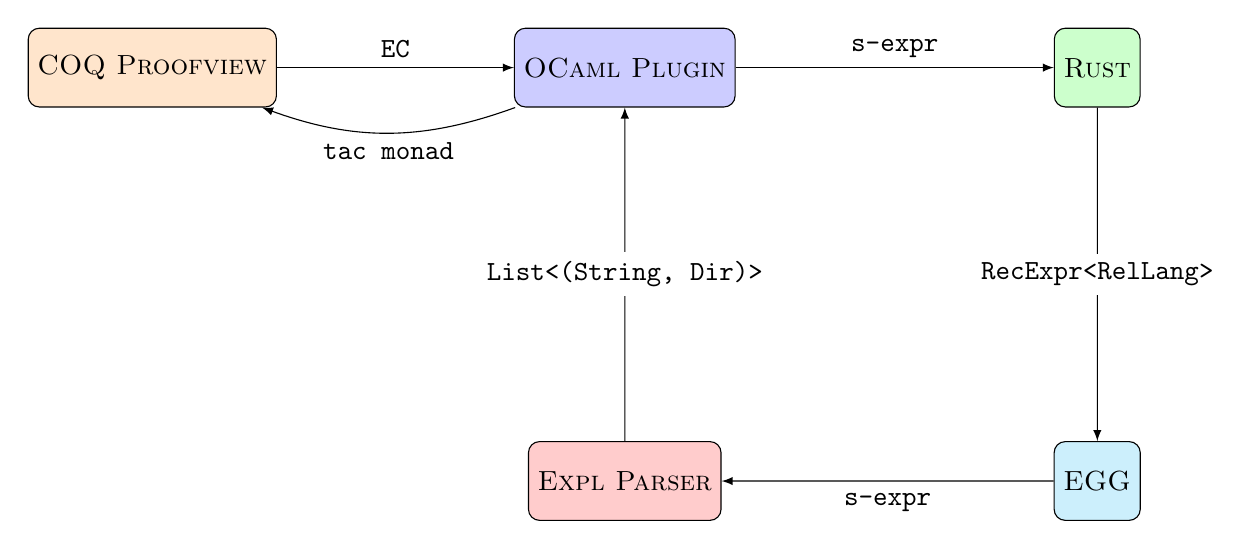
\begin{tikzpicture}[ampersand replacement=\&, scale=1.5]
        \node[rectangle, rounded corners, draw, fill=orange!20, minimum height=1cm] at (0,0) (CP) {\textsc{COQ Proofview}};
        \node[rectangle, rounded corners, draw, fill=blue!20, minimum height=1cm] at (4,0) (OP) {\textsc{OCaml Plugin}};	
        \node[rectangle, rounded corners, draw, fill=green!20, minimum height=1cm] at (8,0) (RUST) {\textsc{Rust}};	
        \node[rectangle, rounded corners, draw, fill=cyan!20, minimum height=1cm] at (8,-3.5) (EGG) {\textsc{EGG}};	
        \node[rectangle, rounded corners, draw, fill=red!20, minimum height=1cm] at (4,-3.5) (EP) {\textsc{Expl Parser}};	

        \draw [-latex] (CP) to node [above, sloped] (TextNode1) {\texttt{EC}} (OP);
        \draw [-latex] (OP) to node [above, sloped] (TextNode1) {\texttt{s-expr}} (RUST);
        \draw [-latex] (RUST) to node [fill=white] (TextNode1) {\texttt{RecExpr<RelLang>}} (EGG);
        \draw [-latex] (EGG) to node [below, sloped] (TextNode1) {\texttt{s-expr}} (EP);
        \draw [-latex] (EP) to node [fill=white] (TextNode1) {\texttt{List<(String, Dir)>}} (OP);
        \draw [-latex] (OP) to[bend left=20] node [below] (TextNode1) {\texttt{tac monad}} (CP);

    \end{tikzpicture}
    \caption{Components of the system}\label{fig:components}
\end{figure}

A term with a proposition to prove is extracted from Coq Proofview using Coq-Api. Expression is parsed into a smaller custom type and  transferred to Rust. Rust makes data ready to be used by egg and runs equality saturation algorithm. After that, the proof is constructed and returned to OCaml, conveniently packed. Finally, OCaml performs changes in Coq Proofview. 

\subsection{Vernacular Commands}\label{sec:vernacular_commands}
To extend Coq's grammar with a new tactic or command, one should write a \texttt{.mlg} file, where the tactic's syntax is defined. Consider an example: 

\vspace{0.5cm}
\begin{lstlisting}[language=ocaml_vernac, label=lst:mlg_example]
    DECLARE PLUGIN "coq-via-egg-plugin.plugin"

    VERNAC COMMAND EXTEND cegg_config CLASSIFIED AS QUERY
    | [ "Cegg" "config" reference(r) ] -> { ... } 
    END

    TACTIC EXTEND cegg_solve
    | [ "Cegg" "solve" ] -> { ... } (* Paring and interpretation rule *)
    END
\end{lstlisting}

In listing~\ref{lst:mlg_example}, we define a command called \texttt{cegg\_config} and a tactic called \texttt{cegg\_solve}. A command is marked as \texttt{QUERY}, meaning it is a \textit{pure} function. Otherwise it would have been marked as \texttt{SIDEFF}. 
\begin{definition}[Pure function]
    A pure function is a function where the return value is only determined by its input values, without observable side effects. 
\end{definition}
After the \texttt{|} symbol, we define the parsing rule and the the interpretation rule, separated by \texttt{->}. The parsing rule itself is a set of terminals that are matched against a string of tokens. The interpretation rule is a function that is called when the parsing rule is matched. More on the \texttt{.mlg} file format can be found in the Coq's plugin guide~\footnote{\href{https://github.com/coq/coq/blob/master/doc/plugin\_tutorial/tuto2/src/g\_tuto2.mlg}{https://github.com/coq/coq/blob/master/doc/plugin\_tutorial/tuto2/src/g\_tuto2.mlg}}.

\subsection{OCaml plugin}
When our tactic is called from inside the Coq proof, firstly, we need to extract the goal. Consider an example: 

\vspace{0.5cm}
\begin{lstlisting}[language=coq]
Lemma example (r : relation A) : 
    r^* ;; r^? (@\equiv@) r^*.
Proof.
    Cegg solve eq. 
\end{lstlisting}

When we enter the interactive proof process, we see the following proof state: 

\vspace{0.5cm}
\begin{lstlisting}[language=coq]
    A : Type 
    r : relation A
    ============================
    r^* ;; r^? (@\equiv@) r^*
\end{lstlisting}

Current hypothesises are located above the line and the conclusion of the goal --- below. To interact with Coq from OCaml, we use the Coq-Api\footnote{\href{https://coq.github.io/doc/V8.16.0/api/coq-core/index.html}{https://coq.github.io/doc/V8.16.0/api/coq-core/index.html}}, which provides a widest functionality. To extract that information about the goal in OCaml we first enter the Proofview monad.

\begin{definition}[Monad]
    Monads serve as a representation of computations. Consider a computation to be similar to a function that transforms an input to an output, but with an additional component. This component represents the effect that the function has as a consequence of being executed.
\end{definition}

In the following function \texttt{t} denotes the goal. \texttt{enter} applies the goal-dependent tactic, with \texttt{(t -> unit tactic)} type in each goal independently. 

\vspace{0.5cm}
\begin{lstlisting}[language=ocaml]
    val enter : (t -> unit tactic) -> unit tactic
\end{lstlisting}

Now we see that our tactic, all in all, should be a function that takes goal (\texttt{Proofview.Goal.t}) as input and return a tactic monad (\texttt{unit tactic}). When we have such a function, \texttt{enter} will apply it to each goal. 

Having a \texttt{gl {:} Proofview.Goal.t} as input, we need to split it into the conclusion, hypotheses and the environment, using functions \texttt{concl}, \texttt{hyps} and \texttt{env} respectively. The most import for us is the \texttt{concl}, which we will get. It has a \texttt{EConstr.constr}, which is the most important datatype in Coq, namely the kernel term. It is used to represent expressions, which are built using a set of constructors that correspond to the different types and operations. 

% TODO: Жидокато в конце написал, надо лучше
Our next task is to prepare the conclusion for the \texttt{egg} use. \texttt{Econstr.t} (similar to \texttt{Econstr.constr}) has a huge list of constructors, but we are not expecting to handle most of them. For example, constructors such as \texttt{Forall} or \texttt{LetIn} are not something we expect to see in a proposition about relations. From the limitations of what kind of rules we can pass to \texttt{egg} we can infer that we want to handle particular relations and various operations on them, i.e.\ applications of functions. Moreover, after analysing the Hahn library and the imm code base, we have decided to add some concrete relations as constants: An empty relation, denoted as \texttt{(fun\_ \_ => False)}, which means that for any two elements of the given set are related, and a full relation, denoted as \texttt{(fun \_ \_ => True)}. Thereby the constructors we are interested in are as follows: 

\vspace{0.5cm}
\begin{lstlisting}[language=ocaml]
    type Econstr.constr = 
        | App of 'constr * 'constr array
        | Var of Names.Id.t
        | Lambda of Names.Name.t Context.binder_annot * 'types * 'constr
        | Ind of Names.inductive * 'univs (* Inductive constructors, e.g. True or False *)
\end{lstlisting}

The conclusion of the goal is splitted by the equivalence sign into the \texttt{lhs} and the \texttt{rhs} of the equation. Both sides are individual \texttt{Econstr.t}'s that will be passed to Rust as two terms separately. \texttt{Econstr.t} is parsed into a smaller type. If unexpected constructors occur in the expression, exception is raised and a error is shown to the user. Data type is an s-expression over strings, with an addition of lambdas: 

\vspace{0.5cm}
\begin{lstlisting}[language=ocaml]
    type goal_s_expr =
        | Symbol of string
        | Application of string * goal_s_expr list
        | Lambda of goal_s_expr * goal_s_expr
\end{lstlisting}

Next step is to pass an object of type \texttt{goal\_s\_expr} to Rust for further processing. We use the \texttt{ocaml-rs}~\cite{OCaml_rust_ffi} Rust library to set up communication between OCaml and Rust. Similar type as \texttt{goal\_s\_expr} is defined in Rust: 

\vspace{0.5cm}
\begin{lstlisting}[language=rust, style=colouredRust]
    pub enum GoalSExpr {
        Symbol(String),
        Application(String, LinkedList<GoalSExpr>),
        Lambda(Box<GoalSExpr>, Box<GoalSExpr>),
    }
\end{lstlisting}

\subsection{Using Egg}
Now we want to define an e-graph, which \texttt{egg} will operate with. EGraphs are parameterized over the Language given by the user. We define a language in the same notation as introduced in Section~\ref{egraphs}. We denote the following language, which represents operations on relations: 

\vspace{0.5cm}
\begin{lstlisting}[language=rust, style=colouredRust]
    define_language! {
        pub enum RelLanguage {
            "top" = Top,                  // Full relation
            "bot" = Bot,                  // Empty relation
            "complete_set" = CompleteSet, // Full set
            ";;" = Seq([Id; 2]),          // Relational composition
            "+" = CT(Id),                 // Transitive closure 
            "?" = RT(Id),                 // Reflexive closure
            "*" = CRT(Id),                // Transitive-reflexive closure
            "eqv_rel" = Eqv(Id),          // Equivalence relation 
            "clos_sym" = CS(Id),          // Symmetric closure
            "-1" = Transpose(Id),         // Relational transposition 
            "clos_refl_sym" = CRS(Id),    // Symmetric-reflexive closure
            "||" = Union([Id; 2]),        // Union of relations 
            "&&" = Inter([Id; 2]),        // Intersection of relations
            "sminus" = SetMinus([Id; 2]), // Set difference
            Symbol(Symbol),               // Concrete relations
        }
    }
\end{lstlisting}

Rust component recieves two terms (\texttt{lhs} and \texttt{rhs} of the goal conclusion) as input and translates both of them into \texttt{RelLanguage}. Then \texttt{egg} builds an e-graph for the \texttt{lhs}. After that, we aim to saturate the e-graph with equivalences, so that it will represent a set of relations, equivalent to the \texttt{lhs}. Equality saturation algorithm is parameterized with a set of rules. We take useful theorems about relations from the Hahn library and define a rewriting system in \texttt{egg}'s notation:

\vspace{0.5cm}
\begin{lstlisting}[language=rust, style=colouredRust]
    vec![
        rewrite!("ct_rt"; "(;; (+ ?r) (* ?r))" <=> "(+ ?r)"),
        rewrite!("rt_ct"; "(;; (* ?r) (+ ?r))" <=> "(+ ?r)"),
        rewrite!("cr_seq"; "(;; (? ?r) ?r')" <=> "(|| ?r' (;; ?r ?r'))"),
        // ...
    ]
\end{lstlisting}

A rewriting system consits of named rules with patterns to search for in the e-graph and terms to replace them with. \texttt{?r} denotes an arbitrary term named \texttt{r} and the \texttt{<=>} sign is a syntactic sugar for a pair of rules: \texttt{a <=> b} is equivalent to \texttt{a => b} and \texttt{b => a}. Currently, we have chosen 51 rules for the system. When the set of rewrites is provided we run equality saturation algorithm. It iteratively searches for a \texttt{lhs} pattern to apply and expands the e-graph. More on equality saturation in \texttt{egg} could be found in the paper~\cite{egg} and a pseudocode is given in \texttt{egg}'s tutorial~\footnote{\href{https://docs.rs/egg/latest/egg/tutorials/\_01\_background/index.html}{https://docs.rs/egg/latest/egg/tutorials/\_01\_background/index.html}}. Having a saturated graph, to check two terms for equivalence we can call a built-in function \texttt{egraph.equivs(expr1, expr2)}. 

\subsection{Naive implementation complexity}
If we follow the naive algorithm strategy to build an e-graph, we can bump into a problem. Unfortunately, choice of the rules has a massive impact on performance. Even though e-graph as a data structure was designed to store potentially infinite number of terms, some rule combinations can lead to uncontrolled growth. Consider an example: 
 
\vspace{0.5cm}
\begin{lstlisting}[language=rust, style=colouredRust, label=lst:just_rtb]
    vec![
        rewrite!("rt_begin"; "(;; (? ?r) (* ?r))" <=> "(* ?r)"),
    ]
\end{lstlisting}

If we have a rewrite system with just one rule: Listing~\ref{lst:just_rtb}, and we build an e-graph for expression \texttt{r* {;;} r?}, we get a tiny e-graph with 5 nodes, e-graph is shown in Figure~\ref{fig:just_rtb}.

\begin{figure}[h]
    \centering
    \includegraphics[width=0.25\textwidth]{img/rules_important_egraph1.pdf}
    \caption{Saturated e-graph for \texttt{r* {;;} r?} with just one rule}\label{fig:just_rtb}
\end{figure}

However, if we add another rule to the system, the saturation algorithm will not terminate, if we do not set the node/iteration limit. We add an assosiativity rule for the \texttt{;;} operator, for simplicity it will be unidirectional:

\vspace{0.5cm}
\begin{lstlisting}[language=rust, style=colouredRust, label=lst:just_rtb]
    vec![
        rewrite!("rt_begin"; "(;; (? ?r) (* ?r))" <=> "(* ?r)"),
        rewrite!("seqA"; "(;; ?a (;; ?b ?c))" => "(;; (;; ?a ?b) ?c)"),
    ]
\end{lstlisting}

With assosiativity, e-graph explodes with new e-classes, that cannot be defined recursively anymore. For example, we get the following set of equivalences: 
\begin{align*}
    \texttt{r*} &\boldsymbol{\equiv} \highlight{blue!30}{\texttt{(r? ;; (r? ;; r?))}} \texttt{;; r*} \\ 
       &\boldsymbol{\equiv} \highlight{blue!30}{\texttt{r?}} \texttt{;; r*} \\ 
       &\boldsymbol{\equiv} \highlight{blue!30}{\texttt{(r? ;; r?)}} \texttt{;; r*} \\ 
       &\boldsymbol{\equiv} \highlight{blue!30}{\texttt{((r? ;; r?) ;; (r? ;; r?))}} \texttt{;; r*} \\ 
\end{align*}

The highlighted subterms in the left parts of the expressions are not equivalent to each other, but they appear in the e-graph during the saturation. 

All in all, the problem is as follows. Expanding rules in tandem with rules that reorder nodes, as commutativty or associativity, can lead to an infinite growth of the e-graph. There are several ways to solve this problem. We have came up with various approaches and will discuss them in detail in Section~\ref{sec:proof_strategies}. Some of the strategies are implemented in our plugin and are available for the user.

\subsubsection{Proof Strategies}\label{sec:proof_strategies}
A less general, but more efficient solution may be to manually schedule, how much particular rules should be applied. If we are trying to prove that \texttt{a} $\boldsymbol{\equiv}$ \texttt{b} and to do so we build an e-graph for \texttt{a} and search for \texttt{b} in it, we can use ``expanding'' rules only for terms that are smaller then \texttt{b}. However, in this thesis, we will focus on more general, but more heuristic approaches. We are still working on providing the user with various trade-offs between efficiency and completeness, all of which can be easily toggled within the plugin. 

All solutions assume that we completely opt out bidirectional rules and orient all of them in the direction of the smaller term. It shrinks the range of problems we can solve, but significantly reduces the time complexity of the algorithm. To prove \texttt{a} $\boldsymbol{\equiv}$ \texttt{b}, we can build an e-graph for \texttt{a} and search for \texttt{b} in it and vice versa. Alternatively, we can build both e-graphs and check their intersection to be non-empty. If we find an element that is equivalent to both \texttt{a} and \texttt{b}, we can conclude that \texttt{a} $\boldsymbol{\equiv}$ \texttt{b} and construct a proof.

\subsection{Retrieving proofs in Coq}
After we finish saturating the e-graph and find out whether two expressions are equivalent in it, we can use \texttt{egg}'s \texttt{explain\_equivalence(expr1, expr2)} function to get the proof. The output will be a series of s-expressions annotated with the rewrite being performed. Consider an example, showing how \texttt{(/ (* (/ 2 3) (/ 3 2)) 1)} (or $(\frac{2}{3} \cdot \frac{3}{2}) / 1$) can be simplified to \texttt{1}:

\vspace{0.5cm}
\begin{lstlisting}[language=rust, style=colouredRust]
    (/ (* (/ 2 3) (/ 3 2)) 1)
    (Rewrite<= div-one (* (/ 2 3) (/ 3 2)))
    (* (Rewrite=> unsafe-invert-division (/ 1 (/ 3 2))) (/ 3 2))
    (Rewrite=> cancel-denominator 1)
\end{lstlisting}

This sequence of s-expressions is parsed to a list of tuples with names of theorems to apply and directions (\texttt{forward} or \texttt{backward}) in which to apply them. This data is returned as to OCaml, OCaml consequently applies \texttt{rewrite} tactic with a given theorems inside the goal, and concludes the proof using \texttt{reflexivity} tactic. This is how we automate the proof of equivalence of two expressions in our plugin.

\subsection{Plugin configuration}
By that moment we have described the ideas and the most important parts behind the algorithm that checks two terms for equivalence using \texttt{egg}. Along with that, the plugin supports the functionality to provide \texttt{egg} with user pre-defined rewriting rules, in compliment to the ones we have defined ourselves. For that, the vernacular command (more on vernacular commands in Section~\ref{sec:vernacular_commands}) \texttt{cegg\_config} is provided. The set of theorems with which we configured the egg consists of statements about abstract relationships. In addition to them, in order to prove more substantial facts, it is necessary to use axioms of specific relationships with a stable meaning. Such axioms are usually combined into a set called \emph{well-formed} (WF). Consider the following example.

\vspace{0.5cm}
\begin{lstlisting}[language=coq, label=lst:wf_example, caption={Well-formed example},captionpos=b]
    Variable rf : A -> A -> Prop.
    Variable mo : A -> A -> Prop.
    Notation "'fr'" := ( rf(@${}^{-1}$@) ;; mo).

    Record Wf :=
    { 
        rf_mo : rf ;; mo (@$\equiv$@) (@$\varnothing$@) ;
        rf_rf : rf ;; rf (@$\equiv$@) (@$\varnothing$@) ;
        mo_rft : mo ;; rf(@${}^{-1}$@) (@$\equiv$@) (@$\varnothing$@) ;
        mo_fr : mo ;; fr (@$\equiv$@) (@$\varnothing$@) ; 
        fr_fr : fr ;; fr (@$\equiv$@) (@$\varnothing$@) ;
    }.

    Cegg config Wf.
\end{lstlisting}

The object with axioms is created, then passed to OCaml plugin, WF is checked to contain only relational equivalences, then it is tramsferred to Rust, where it is cached in build folder. Afterwards, these axioms would be used along with pre-defined ones to prove theorems.

\subsection{Evaluation}
Unfortunately, we cannot demonstrate usability of the created tool to prove any popular substantive results. An example of such a result could be proving the equivalence of two definitions of the \texttt{eco} relation. Consider a slightly modified Listing~\ref{lst:wf_example}.

\vspace{0.5cm}
\begin{lstlisting}[language=coq, label=lst:eco_example, caption={Eco equivalent definitions}, captionpos=b]
    Variable rf : A -> A -> Prop.
    Variable mo : A -> A -> Prop.
    Notation "'fr'" := ( rf(@${}^{-1}$@) ;; mo).

    Notation "'eco1'" := (rf (@$\cup$@) mo (@$\cup$@) fr)^+.
    Notation "'eco2'" := (rf (@$\cup$@) (mo ;; rf^?) (@$\cup$@) (fr ;; rf^?)).

    Record Wf :=
    { 
        mo_trans : mo ;; mo (@$\subseteq$@) mo ; 
        rf_mo : rf ;; mo (@$\equiv$@) (@$\varnothing$@) ;
        rf_rf : rf ;; rf (@$\equiv$@) (@$\varnothing$@) ;
        mo_rft : mo ;; rf(@${}^{-1}$@) (@$\equiv$@) (@$\varnothing$@) ;
        mo_fr : mo ;; fr (@$\equiv$@) (@$\varnothing$@) ; 
        fr_fr : fr ;; fr (@$\equiv$@) (@$\varnothing$@) ;
    }.

    Implicit Type WF : Wf.

    Lemma eco_eq WF : 
        eco1 (@$\equiv$@) eco2.
    Proof.
\end{lstlisting}

Despite the fact that we need to prove the equivalence of two relations, one of the properties we need to use along the way is \texttt{mo\_trans}, which was added to the WF in Listing~\ref{lst:eco_example}. In the process of proof, we inevitably need to use inclusions of one relation into another, which unfortunately our plugin cannot do automatically. Based on our work, we have reached the conclusion that for verified automated proofs of equivalences, we frequently require to operate with inclusions of relations, which our approach is not capable of. In order to adapt the equality saturation approach to our task, we need to improve the e-graphs so that they can store asymmetric rewrites.

Nevertheless, the created solution can solve simple subtasks and simplify work in a limited set of cases, when all intermediate steps involve only equivalence rewrites, for example, consider taking Listing~\ref{lst:wf_example} and trying to prove the following Lemma: 

\vspace{0.5cm}
\begin{lstlisting}[language=coq]
    Lemma eco_sub WF (r : relation A) :
        (fr (@$\cup$@) mo) ;; (fr (@$\cup$@) mo) (@$\equiv$@) fr ;; mo (@$\cup$@) mo ;; mo.
    Proof.
        rewrite -> seq_union_r.
        rewrite -> seq_union_l.
        rewrite -> fr_fr.
        rewrite -> mo_fr.
        rewrite -> union_false_l.
        rewrite -> union_false_l.
        rewrite -> seq_union_l.
        all: auto.
    Qed.

    Lemma eco_sub' WF (r : relation A) :
        (fr (@$\cup$@) mo) ;; (fr (@$\cup$@) mo) (@$\equiv$@) fr ;; mo (@$\cup$@) mo ;; mo.
    Proof. Cegg solve eq. Qed. 
\end{lstlisting}

It takes 7 rewrite calls to prove this lemma by hand, but it takes only about 4 seconds for our tool to solve it automatically. Here we have used the proof strategy where all rules are bidirectional. Strategies without expanding rules (described in Section~\ref{sec:proof_strategies}) are usually executed in less then 800ms. 